\chapter{Evaluation}
\label{ch:Evaluation}

\abstract{This chapter provides the analysis of the statistics gathered from the final implementations. As stated in the introduction the evaluation considers raw performance characteristics as well as developer productivity. Both areas are evaulated based on statistics from the previous chapter.
}

Preface: All data in this chapter was gathered from a high performance computer by courtesy of the research group Scientific Computing. The machine has access to four 12-core processors and 128 GB of memory. It is therefore ideal to compare shared memory performance on a large scale.

\section{Performance}
\label{sec:Evaluaton::Performance}

In \acrlong{hpc} the most important criteria when evaluating a language is performance. The important statistic that was tracked to compare performance is execution time. The benchmarks that were performed on the development laptop also roughly measured memory usage but that proved difficult to automate on the remote machine. It is therefore not directly included in this final evaluation. The first table shows the benchmark results in varying concurrency scenarios from singlethreaded execution up to 48 calculating in parallel.

\begin{table}[htb]
    \centering
    \begin{tabular}{rccc}
        \toprule
        % Header
            threads/goroutines
            & C
            & Go
            & Rust \\
        \midrule

            1
            & 21:51:18
            & 16:48:19
            & 14:15:06 \\

            2
            & 12:29:56
            & 10:21:36
            & 09:12:47 \\

            4
            & 07:16:34
            & 05:58:35
            & 05:09:56 \\

            8
            & 04:13:04
            & 03:01:54
            & 02:49:35 \\

            12
            & 03:17:28
            & 02:06:08
            & 01:55:33 \\

            24
            & 02:06:08
            & 01:13:47
            & 01:03:34 \\

            48
            & 01:21:58
            & 00:53:54
            & 00:44:54 \\

        \bottomrule
    \end{tabular}
    \caption{Execution time of the final applications (100K nodes)}
    \label{tb:final_execution_time}
\end{table}

These results already contain the first real surprise. C that was chosen as a comparitive baseline, since it is one of the two big programming languages in \gls{hpc}, is the slowest of the three compared languages in all configurations. In contrast the preliminary benchmarks on the development laptop showed C while not ahead at least on second place in the performance comparison. As briefly mentioned in the \hyperref[subsec:Implementation::ClusterPreparation::C]{previous chapter} this performance regression might have been caused by the two unoptimized libraries that were compiled on the development laptop and copied to the cluster. However this shows that C is still very much compiler and machine dependent.

In contrast the Go binary that was also compiled on the development laptop was executed without any changes on the target machine and shows great result even reaching similar performance to Rust in the high concurrency configurations. This shows that a garbage collected language is not immediately unsuitable for use in \gls{hpc}. Combined with the portability caused by full static linking Go might very well be suited for cluster computations on nodes with a minimum of system libraries installed.

Finally Rust demonstrates that it might be a competent successor to C in \gls{hpc}. It is the fastest language out of the compared three across all scenarios while provding additional memory safety through its unique typesystem. It prevented multiple errors from compiling in the Rust implementation throughout the whole development process. On one occasion it even revealed an error which had gone unnoticed in both C and Go. This really highlights how static analysis can provide safety without sacrificing performance.

Another important statistic to compare is the parallel speedup. A slow execution time alone does not mean a language is completely unfit for \gls{hpc} because the implementation might simply be flawed to begin with. If this is the case the application can still offer above average speedups making it viable for high concurrency scenarios. The following table lists the achieved speedup for each language in the same configurations as above.

\begin{table}[htb]
    \centering
    \begin{tabular}{rccc}
        \toprule
        % Header
            threads/goroutines
            & C
            & Go
            & Rust \\
        \midrule

            1
            & \hspace{6pt}1.0000
            & \hspace{6pt}1.0000
            & \hspace{6pt}1.0000 \\

            2
            & \hspace{6pt}1.7486
            & \hspace{6pt}1.6221
            & \hspace{6pt}1.5469 \\

            4
            & \hspace{6pt}3.0037
            & \hspace{6pt}2.8119
            & \hspace{6pt}2.7590 \\

            8
            & \hspace{6pt}5.1816
            & \hspace{6pt}5.5432
            & \hspace{6pt}5.0424 \\

            12
            & \hspace{6pt}6.6406
            & \hspace{6pt}7.9941
            & \hspace{6pt}7.4003 \\

            24
            & 10.3961
            & 13.6659
            & 13.4520 \\

            48
            & 15.9980
            & 18.7072
            & 19.0445 \\

        \bottomrule
    \end{tabular}
    \caption{Parallel speedup of the final applications (100K nodes)}
    \label{tb:final_speedup}
\end{table}

Again the results are interesting for multiple reasons. C scales very well up to four threads but falls off quite heavily. Rust and Go are evenly matched with Go scaling better up to the final benchmark with 48 threads where it gets beaten slightly by Rust. It would be interesting to see the trend continue here but unfotunately the target machine ``only'' offered 48 logical cores. C' strong scaling in the lower thread counts shows OpenMP's efficiency in generating threaded code for common desktop scenarios. In the high concurrency configurations though the scaling diminishes resulting in a big discrepancy of about 3 (\textasciitilde13\%). For these use cases it might be worthwhile to implement custom parallelization with \textit{pthreads}.\fnote{\url{http://pubs.opengroup.org/onlinepubs/9699919799/basedefs/pthread.h.html}} This approach will most likely result in much higher development time but might yield better performance results for higher thread counts.

Rust and Go scale both comparably well. Although the final speedup of about 19 is not great for 48 threads it is still a serious improvement about the serial version. It is also important to note that the threads share the work with statically which means there is no load balancing once the threads are started. This results in some threads exiting early effectively reducing the speedup. To solve this the work could be dynamically distributed for example through a queue like construct which threads use to retrieve new tasks. A possible implementation could be channel based as both Go and Rust offer those as part of the standard library.

\section{Additional metrics / productivity}
\label{sec:Evaluation::Metrics}

Next to performance the second main area evaluated in this thesis is developer productivity. The two criteria tracked to compare this category are \gls{sloc} count and development time. While the \gls{sloc} count is certainly not the best code quality metric it allows for some basic conclusions. Less lines can contain potentially less errors, lowering maintenance costs, and \textit{should} take less time develop. Although this is obviously not always true but the following graphs mostly confirm this correlation for the evaluated implementations.

\begin{figure}[htb]
    \centering
    \makebox[\textwidth][c]{%
        \subfloat[Development time]{%
        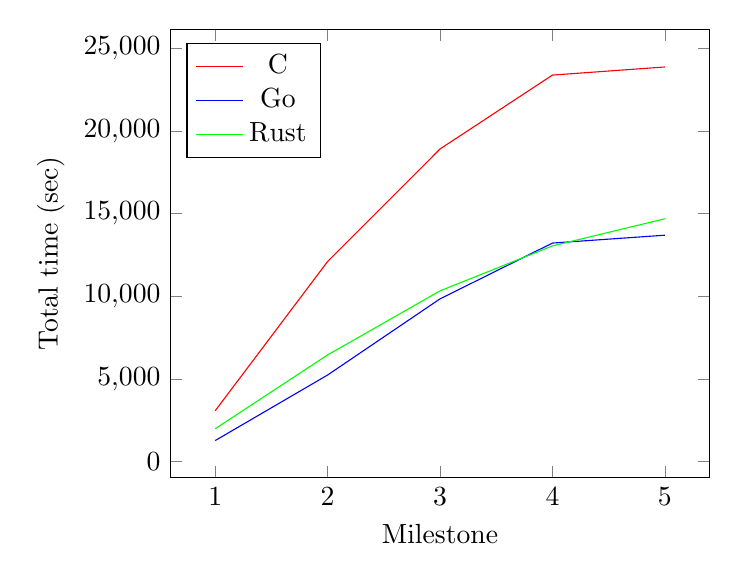
\begin{tikzpicture}
            \begin{axis}[
                xlabel={Milestone},
                ylabel={Total time (sec)},
                xtick={1,2,3,4,5,6},
                scaled y ticks = false,
                ylabel near ticks,
                legend pos=north west]

                \addplot[red] plot coordinates {
                  (1,3078)
                  (2,12110)
                  (3,18920)
                  (4,23392)
                  (5,23883)};
                \addlegendentry{C}

                \addplot[color=blue] plot coordinates {
                  (1,1276)
                  (2,5242)
                  (3,9851)
                  (4,13227)
                  (5,13703)};
                \addlegendentry{Go}

                \addplot[color=green] plot coordinates {
                  (1,1989)
                  (2,6457)
                  (3,10335)
                  (4,13055)
                  (5,14698)};
                \addlegendentry{Rust}

            \end{axis}
        \end{tikzpicture}
        }
        \subfloat[SLOC counts]{%
        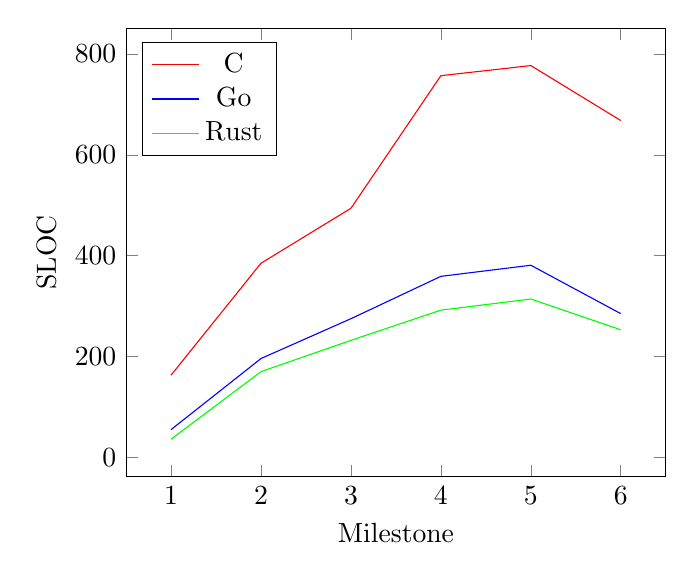
\begin{tikzpicture}
            \begin{axis}[
                xlabel={Milestone},
                ylabel={SLOC},
                xtick={1,2,3,4,5,6},
                legend pos=north west]

                \addplot[red] plot coordinates {
                  (1,163)
                  (2,385)
                  (3,494)
                  (4,757)
                  (5,777)
                  (6,668)};
                \addlegendentry{C}

                \addplot[color=blue] plot coordinates {
                  (1,55)
                  (2,196)
                  (3,275)
                  (4,359)
                  (5,381)
                  (6,285)};
                \addlegendentry{Go}

                \addplot[color=green] plot coordinates {
                  (1,36)
                  (2,170)
                  (3,232)
                  (4,292)
                  (5,314)
                  (6,253)};
                \addlegendentry{Rust}

            \end{axis}
        \end{tikzpicture}
        }
    }
    \caption{Productivity metrics across the various milestones}
    \label{fig:productivity_metrics}
\end{figure}

The sixth milestone in the \gls{sloc} count graph measured the final stripped down versions as introduced in \autoref{sec:Implementation::ParallelBenchmark}. It is not included in the development time comparison as this statistic was not tracked.
